\documentclass[10pt,a4paper]{article}

\usepackage[main=french]{babel}
\usepackage[T1]{fontenc}
\usepackage{geometry}
\usepackage{changepage}
\usepackage{amsmath,amssymb,amsfonts,helvet,color}
\usepackage{amsthm}%\usepackage[pdftex]{graphicx}
\usepackage{graphicx}
\usepackage{graphics}
\usepackage{indentfirst}
\usepackage{amsmath,amssymb,amsfonts,subeqnarray}
\usepackage[dvipsnames]{xcolor}
\usepackage{listings}
\usepackage{enumitem}
\usepackage{bm}  % Pour le texte en gras
\usepackage{xcolor}
\usepackage[normalem]{ulem}
\usepackage{pdfpages}
\usepackage{subcaption}
\usepackage{datatool}
\usepackage{tabularx}
\usepackage{setspace}

\usepackage{float}


\usepackage{geometry}
\geometry{top=3cm, bottom=3cm, left=2.25cm , right=2.25cm}
\usepackage{hyperref}
\hypersetup{
    colorlinks=true,
    linkcolor=BlueViolet,
    filecolor=OrangeRed,      
    urlcolor=blue,
    }
\title{Rapport de projet CPU/GPU}
\author{\\Matthieu PETIT\\Djemsay Morvan\\Ulysse Caromel\\\\\\
Encadrant : Mariko Dunseath\\\\\\}

\begin{document}

\setstretch{1.3}


% \maketitle

\begin{titlepage}

    \begin{center}
        \begin{center}
            
\includegraphics[height=2.5cm]{../Images/univ-rennes1.png}
            
        \end{center}
        \begin{center}
            \textbf{UNIVERSITE RENNES 1 }
        \end{center}
        \textsc{\Large }\\[2.5cm]
    % Title
    \rule{\linewidth}{0.3mm} \\[0.4cm]
    { \huge \bfseries Rapport de fin de projet CPU/GPU \\[0.4cm] }
    \rule{\linewidth}{0.3mm} \\[3cm]
    
    
    % Author and supervisor
    \noindent
    \begin{center}
        \textbf{Petit} Matthieu\\
        \textbf{Caromel} Ulysse\\
        \textbf{Morvan} Djemsay\\
    \end{center}
        
    \color{black}
    \centering
    \vfill
    \large \textbf{Encadrant} - ~\textsc{Mariko Dunseath} 
    
    \vfill
    
    % Bottom of the page
    {\textbf{\large {Année universitaire} 2023-2024}}
    
    \end{center}
\end{titlepage}

\newpage

\tableofcontents

\newpage

\section{Partie théorique}

\subsection{Méthode de quadrature de Simpson}

La méthode de quadrature de Simpson est une technique numérique utilisée pour estimer l'intégrale numériquement. Elle est basée sur l'approximation d'une fonction par un polynôme quadratique entre chaque paire de points adjacents.

Supposons que nous ayons une fonction $f(x)$ que nous voulons intégrer sur l'intervalle $[a, b]$. La méthode de Simpson divise cet intervalle en sous-intervalles de largeur égale $h = \frac{b - a}{n}$, où $n$ est un nombre pair.

L'approximation de l'intégrale sur chaque sous-intervalle $[x_i, x_{i+2}]$ est donnée par :
\begin{align*}
\int_{x_i}^{x_{i+2}} f(x) \,dx \approx \frac{h}{3} \left[ f(x_i) + 4f(x_{i+1}) + f(x_{i+2}) \right]
\end{align*}

La somme de ces approximations sur tous les sous-intervalles donne l'estimation finale de l'intégrale :
\begin{align*}
\int_{a}^{b} f(x) \,dx \approx \frac{h}{3} \left[ f(a) + 4f(x_1) + 2f(x_2) + \ldots + 2f(x_{n-2}) + 4f(x_{n-1}) + f(b) \right]
\end{align*}

La méthode de Simpson est souvent plus précise que les méthodes de quadrature plus simples comme la méthode des rectangles, car elle prend en compte les variations de la fonction sur chaque sous-intervalle.


\subsection{Méthode de Gauss 2D}


La méthode de quadrature Gaussienne en deux dimensions (Gauss 2D) est utilisée pour estimer numériquement l'intégrale d'une fonction $f(x, y)$ sur une région bidimensionnelle définie par $a \leq x \leq b$ et $c \leq y \leq d$.

Supposons que nous ayons une fonction à intégrer sur cette région. La méthode de Gauss 2D utilise un ensemble de points et de poids associés pour approximer l'intégrale. La formule générale pour cette approximation est donnée par :
\begin{align*}
\iint_{R} f(x, y) \,dx\,dy \approx \sum_{i=1}^{n} \sum_{j=1}^{m} w_{ij} \cdot f(x_i, y_j)
\end{align*}

où $n$ et $m$ sont le nombre de points dans les directions $x$ et $y$, respectivement. Les points $x_i$ et $y_j$ sont les emplacements des points de quadrature, et $w_{ij}$ sont les poids associés à ces points.

Une formule spécifique de quadrature Gaussienne 2D pour un quadrilatère est donnée par :
\begin{align*}
\iint_{R} f(x, y) \,dx\,dy \approx \sum_{i=1}^{n} \sum_{j=1}^{m} w_{ij} \cdot f\left(\frac{1}{2}(1 + \xi_i)x + \frac{1}{2}(1 - \xi_i)y, \frac{1}{2}(1 + \eta_j)x + \frac{1}{2}(1 - \eta_j)y\right)
\end{align*}

où $\xi_i$ et $\eta_j$ sont les points de quadrature et $w_{ij}$ sont les poids associés.

La méthode de quadrature Gaussienne 2D offre une précision supérieure à la quadrature de Gauss unidimensionnelle, et elle est souvent utilisée pour résoudre numériquement des intégrales sur des domaines bidimensionnels complexes.


\subsection{Méthode d'intégration de Monte-Carlo}

La méthode d'intégration de Monte Carlo est une technique utilisée en mathématiques pour estimer des valeurs numériques complexes, notamment les intégrales de fonctions dans des domaines à plusieurs dimensions. Elle repose sur des principes probabilistes et tire son nom du célèbre casino de Monte Carlo à Monaco, associant le hasard à des calculs numériques.

L'idée principale de cette méthode consiste à estimer une valeur en utilisant des échantillons aléatoires dans un domaine donné. Prenons l'exemple d'une intégrale définie sur un domaine $D$ dans le plan. Plutôt que d'utiliser des méthodes traditionnelles d'intégration, on peut estimer la valeur de cette intégrale en générant aléatoirement des points dans $D$.

Imaginons que nous voulions calculer l'intégrale $I = \int\int_{D} f(x,y) \, dx \, dy$. La méthode de Monte Carlo fonctionne approximativement comme suit :

\begin{enumerate}
    \item Génération de points aléatoires : On génère un grand nombre de points aléatoires $(x_i, y_i)$ dans le domaine $D$ selon une distribution choisie (souvent uniforme ou gaussienne).
    \item Évaluation de la fonction : On évalue la fonction $f(x,y)$ pour chaque point $(x_i, y_i)$.
    \item Calcul de la moyenne pondérée : On calcule la moyenne des valeurs de $f(x,y)$ évaluées pour les points générés et on multiplie cette moyenne par la mesure de l'ensemble $D$. Cette mesure est souvent estimée par le rapport entre le nombre de points dans $D$ et le nombre total de points générés.
\end{enumerate}

La formule d'estimation de Monte Carlo pour l'intégrale devient alors :
$$I \approx A \cdot \frac{1}{N} \sum_{i=1}^{N} f(x_i, y_i)$$
Où $A$ est la mesure de $D$, $N$ est le nombre de points générés et $(x_i, y_i)$ sont les coordonnées des points aléatoires.

L'avantage clé de cette méthode est sa flexibilité et sa capacité à traiter des problèmes complexes dans des espaces à dimensions élevées. Cependant, sa précision dépend fortement du nombre de points aléatoires générés : plus le nombre de points est élevé, plus l'estimation de l'intégrale sera précise, mais cela peut nécessiter beaucoup de ressources computationnelles.

La méthode de Monte Carlo offre une approche probabiliste puissante pour estimer numériquement des quantités complexes en utilisant des échantillons aléatoires. Son utilisation s'étend dans de nombreux domaines, de la physique à la finance, en raison de sa flexibilité et de sa capacité à traiter des problèmes difficiles à résoudre analytiquement.


\section{Outils utilisés}

\subsection{Open MP (CPU)}

OpenMP (Open Multi-Processing) est une API (Interface de Programmation Applicative) qui facilite la programmation parallèle en C, C++, et Fortran. Son objectif principal est de permettre aux développeurs d'exploiter les architectures parallèles des processeurs multi-cœurs de manière simple et portable.

Voici quelques points clés à propos d'OpenMP :

\begin{itemize}

    \item \textbf{Parallelisme explicite :} OpenMP permet aux programmeurs d'exprimer le parallélisme dans leur code de manière explicite à l'aide de directives de compilation. Ces directives sont des annotations spéciales ajoutées au code source.
    
    \item \textbf{Directives pragmatiques :} Les directives OpenMP sont écrites sous forme de commentaires pragmatiques qui sont ignorés par les compilateurs qui ne supportent pas OpenMP. Cela permet au code source d'être compilé et exécuté sur des machines qui ne prennent pas en charge OpenMP sans erreur.
    
    \item \textbf{Tâches parallèles et boucles :} OpenMP permet la parallélisation de boucles et de sections de code avec des directives telles que \verb|#pragma omp parallel for| pour paralléliser une boucle, ou \verb|#pragma omp parallel sections| pour diviser le code en sections parallèles.
    
    \item \textbf{Gestion automatique de l'ordonnancement :} OpenMP offre une gestion automatique de l'ordonnancement des tâches parallèles, simplifiant ainsi la tâche du programmeur en ce qui concerne la gestion des threads et l'ordonnancement des tâches.
    
    \item \textbf{Support multi-plateforme :} OpenMP est supporté par de nombreux compilateurs sur différentes plates-formes, ce qui rend le code portable entre différentes architectures.

\end{itemize}


En résumé, OpenMP est une solution efficace pour ajouter du parallélisme aux applications existantes sans avoir à réécrire complètement le code. Cela facilite la création de programmes performants sur des architectures multi-cœurs.


\subsection{MPI (CPU)}


MPI (Message Passing Interface) est une norme pour la programmation parallèle utilisée pour développer des applications sur des architectures distribuées ou parallèles. Contrairement à OpenMP qui se concentre sur les architectures multi-cœurs partagées, MPI est conçu pour gérer la communication entre différents processus s'exécutant sur des nœuds distincts d'un cluster.

Voici quelques points clés à propos de MPI :

\begin{itemize}
    
    \item \textbf{Modèle de programmation distribuée :} MPI s'appuie sur un modèle de programmation distribuée où chaque nœud d'un système peut avoir sa propre mémoire et exécute son propre processus. Les processus communiquent entre eux à l'aide de messages.
    
    \item \textbf{Passage de messages :} La communication entre les processus est réalisée via le passage explicite de messages. Les processus s'envoient des messages pour échanger des données ou coordonner leurs activités.
    
    \item \textbf{Abstraction des communications :} MPI fournit une abstraction des communications en permettant aux programmeurs d'utiliser des opérations de communication comme \verb|MPI_Send| et \verb|MPI_Recv| pour envoyer et recevoir des messages.
    
    \item \textbf{Point à point et collectif :} MPI prend en charge à la fois les communications point à point (entre deux processus) et les communications collectives (impliquant plusieurs processus). Les opérations collectives incluent des fonctionnalités telles que la diffusion, la réduction, la barrière, etc.
    
    \item \textbf{Indépendance d'architecture :} Comme OpenMP, MPI est conçu pour être indépendant de l'architecture matérielle, ce qui signifie qu'un code MPI peut être exécuté sur divers types de clusters sans nécessiter de modifications significatives.
\end{itemize}


En résumé, MPI est une norme de programmation parallèle qui permet de développer des applications distribuées en utilisant un modèle de passage de messages. Il est largement utilisé dans le domaine de la simulation, de l'analyse de données massives et d'autres domaines nécessitant une puissance de calcul parallèle sur des clusters de machines.


\subsection{CUDA (GPU)}

CUDA (Compute Unified Device Architecture) est une architecture de calcul parallèle développée par NVIDIA. Elle permet d'utiliser les GPU (Graphical Processing Unit) pour accélérer des tâches de calcul intensif. CUDA est particulièrement utilisé pour le calcul parallèle sur les cartes graphiques NVIDIA.

Voici quelques points clés à propos de CUDA :

\begin{itemize}
    
    \item \textbf{Modèle de programmation parallèle sur GPU :} CUDA permet aux programmeurs d'utiliser la puissance de calcul massivement parallèle des GPU. Il s'appuie sur un modèle de programmation parallèle où des threads s'exécutent simultanément sur les cœurs du GPU.
    
    \item \textbf{Kernels CUDA :} Le code CUDA s'exécute sur le GPU sous la forme de kernels. Un kernel est une fonction qui est exécutée par un grand nombre de threads sur le GPU.
    
    \item \textbf{Hétérogénéité :} CUDA permet l'exécution de code sur le CPU (hôte) et le GPU (dispositif) simultanément. Le CPU gère les tâches de coordination et de gestion générale, tandis que le GPU effectue des calculs massivement parallèles.
    
    \item \textbf{Hiérarchie des threads et des blocs :} Les threads CUDA sont organisés en blocs, et les blocs peuvent être organisés en grilles. Cette hiérarchie permet une gestion fine du parallélisme.
    
    \item \textbf{Gestion explicite de la mémoire :} Les programmeurs doivent gérer explicitement le transfert des données entre le CPU et le GPU, ainsi que la gestion de la mémoire sur le GPU (mémoire globale, mémoire partagée, etc.).
\end{itemize}


En résumé, CUDA permet d'exploiter la puissance de calcul des GPU pour accélérer des tâches parallèles. Il offre un modèle de programmation hétérogène avec une gestion explicite de la mémoire et des directives spéciales pour définir des kernels qui s'exécutent sur le GPU. Cette approche est particulièrement efficace pour des tâches intensives en calcul, comme le rendu graphique, la simulation physique, et l'apprentissage profond.

\clearpage
\section{Implémentation et résultats}
On présente ici les résultats pour chaque méthode et chaque bibiliothèque de parallélisation.

Pour chaque méthode, on présente une étude de l'erreur en fonction du nombre de subdivision ainsi qu'une étude du temps en fonction du nombre de subdivision.

Les outils OpenMP et MPI ont été utilisés avec un maximum de 8 processeurs, tandis que pour CUDA, la configuration utilisé est la suivante : 
\begin{itemize}
    \item CPU : i9-13900KF
    \item RAM : 32 Gb
    \item GPU : Nividia RTX-3060
\end{itemize}

On présente ensuite une étude sur le temps d'éxécution en fonction du nombre de subdivision, ainsi qu'une étude sur l'erreur en fonction du nombre de subdivision et cela pour chaque méthode (Simpson, Gauss 2D, Monte Carlo) et pour chaque parallélisation (Cuda, OpenMP, MPI).
Nous affichons dans un premier temps tout les graphiques obtenus, une analyse sera donnée par la suite en partie (\ref{sec:analyse}).


\subsection{Méthode de Simpson}

\subsubsection{Open MP}


  \begin{figure}[H]
    \centering

    \subcaptionbox{Erreur \label{fig:errSimpMP}}{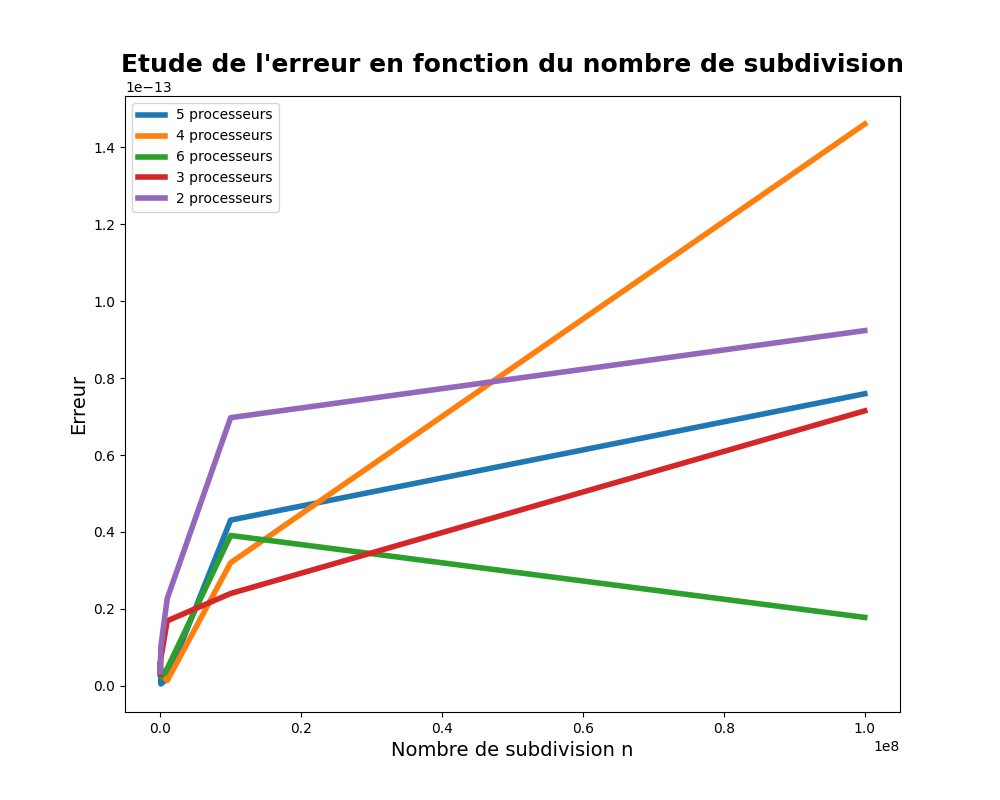
\includegraphics[width=0.45\linewidth]{../Images/error_simp_Op_MP.png}}%
    \hfill 
    \subcaptionbox{Temps \label{fig:timSimpMP}}{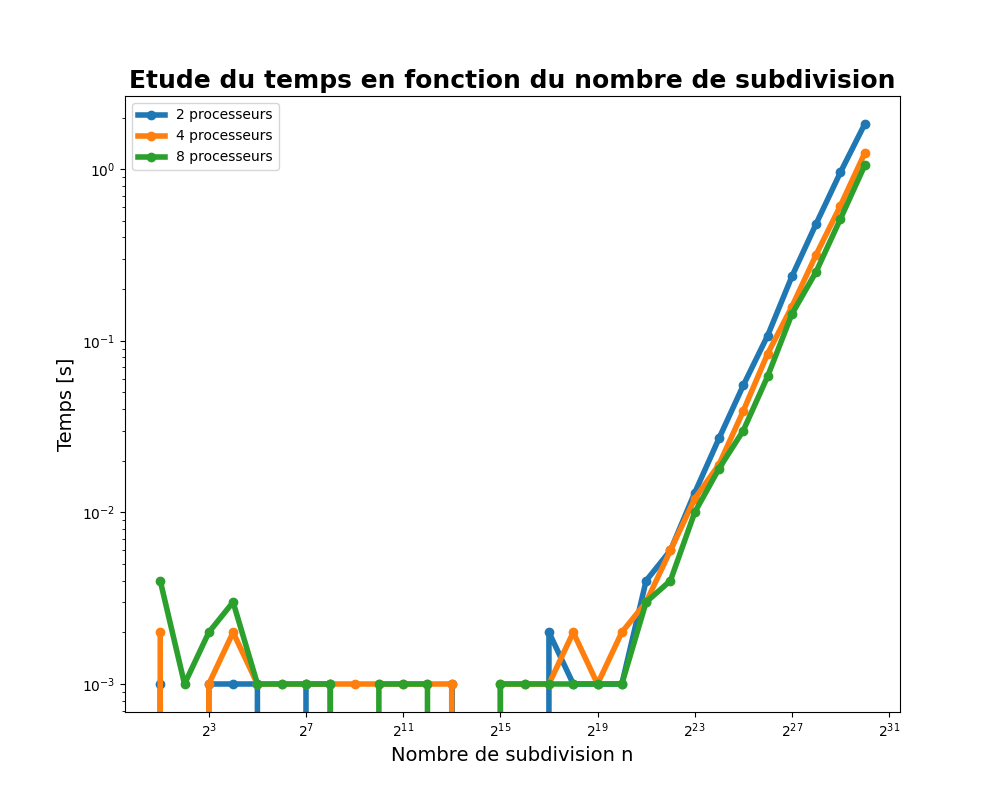
\includegraphics[width=0.45\linewidth]{../Images/time_simp_Op_MP.png}}
  
    \caption{Méthode de Simpson : Open MP}
    \label{fig:simpMP}
  \end{figure}



\subsubsection{MPI}

\begin{figure}[H]
    \centering

    \subcaptionbox{Erreur \label{fig:errSimpMPI}}{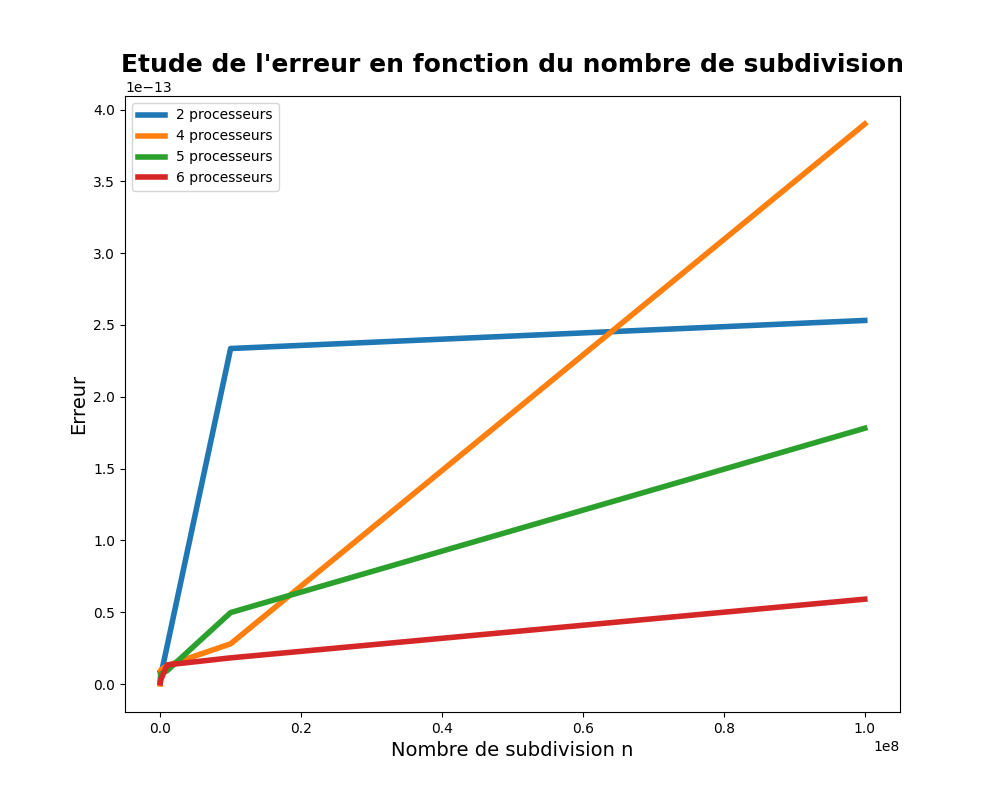
\includegraphics[width=0.45\linewidth]{../Images/error_simp_MPI.png}}%
    \hfill 
    \subcaptionbox{Temps \label{fig:timSimpMPI}}{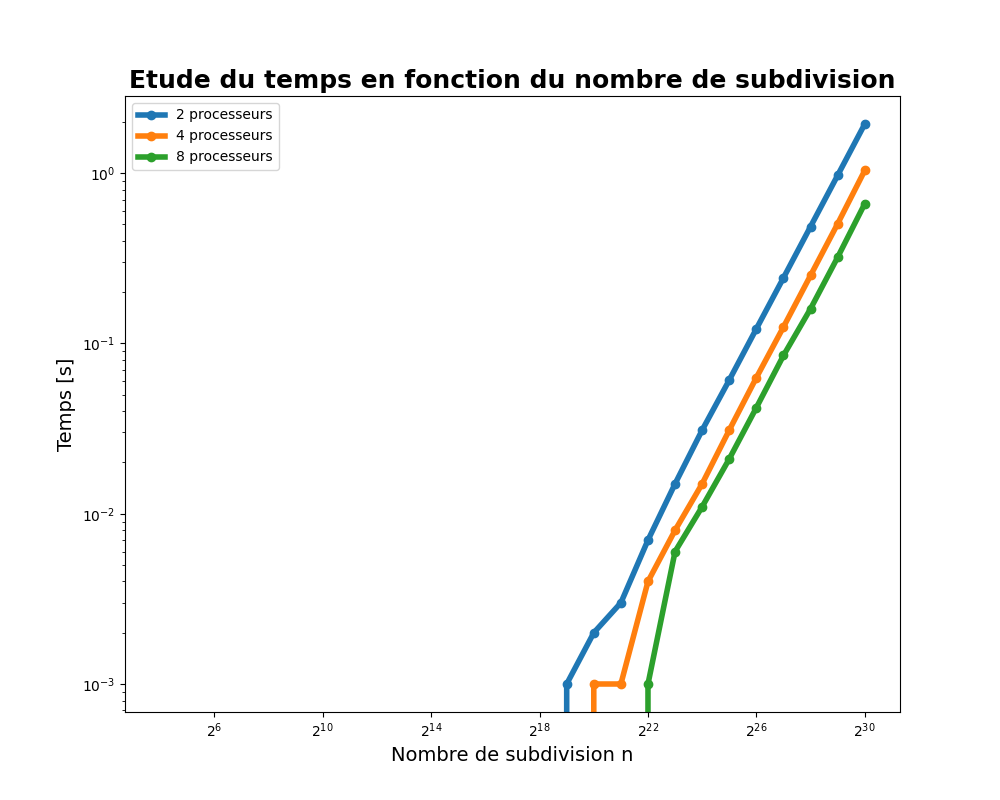
\includegraphics[width=0.45\linewidth]{../Images/time_simp_MPI.png}}
  
    \caption{Méthode de Simpson : MPI}
    \label{fig:simpMPI}
  \end{figure}

\subsubsection{Cuda}
\begin{figure}[H]
    \centering

    \subcaptionbox{Erreur \label{fig:errSimpMPI}}{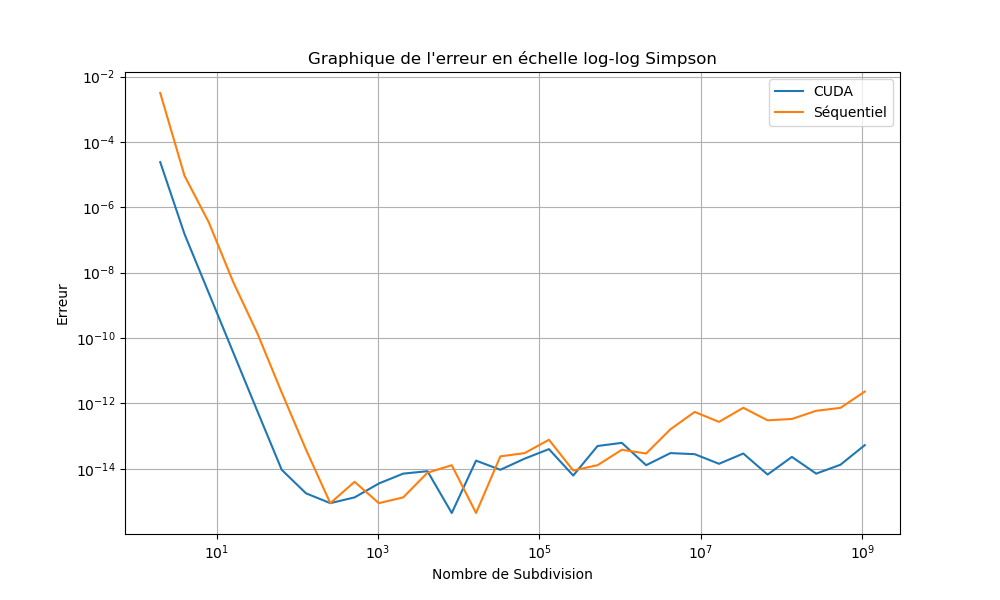
\includegraphics[width=0.45\linewidth]{../Images/error_simpson_cuda.png}}%
    \hfill 
    \subcaptionbox{Temps \label{fig:timSimpMPI}}{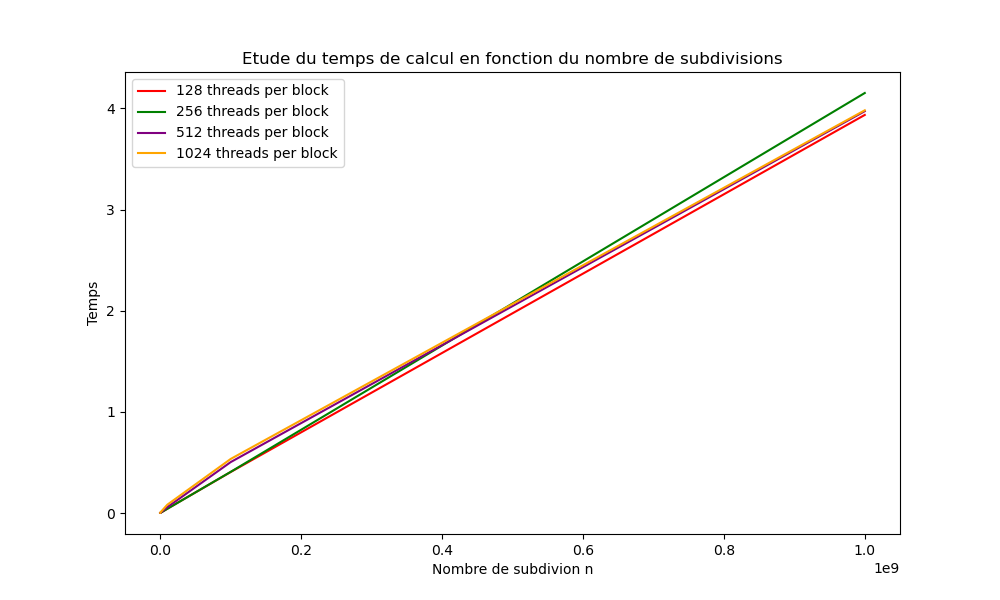
\includegraphics[width=0.45\linewidth]{../Images/time_simpson_cuda.png}}
  
    \caption{Méthode de Simpson : MPI}
    \label{fig:simpMPI}
  \end{figure}

\subsection{Gauss}

\subsubsection{Open MP}

\begin{figure}[H]
    \centering

    \subcaptionbox{Erreur \label{fig:errGaussMP}}{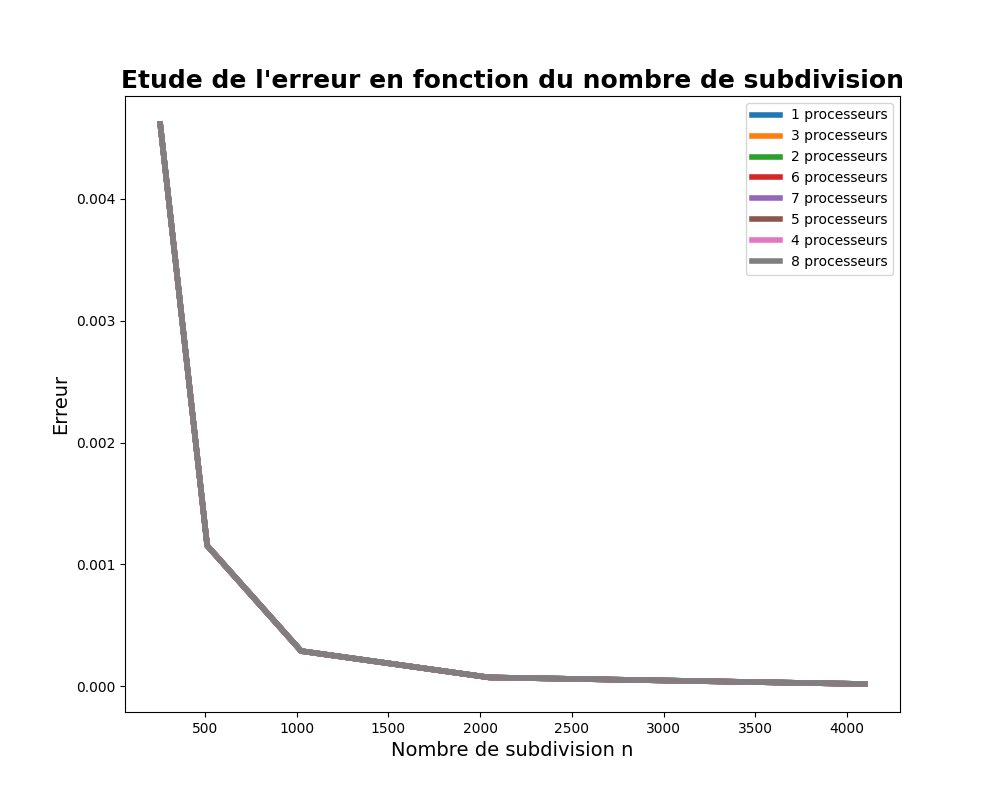
\includegraphics[width=0.45\linewidth]{../Images/error_gauss_Op_MP.png}}%
    \hfill % Ajoute une espace horizontale entre les sous-figures
    \subcaptionbox{Temps \label{fig:timGaussMP}}{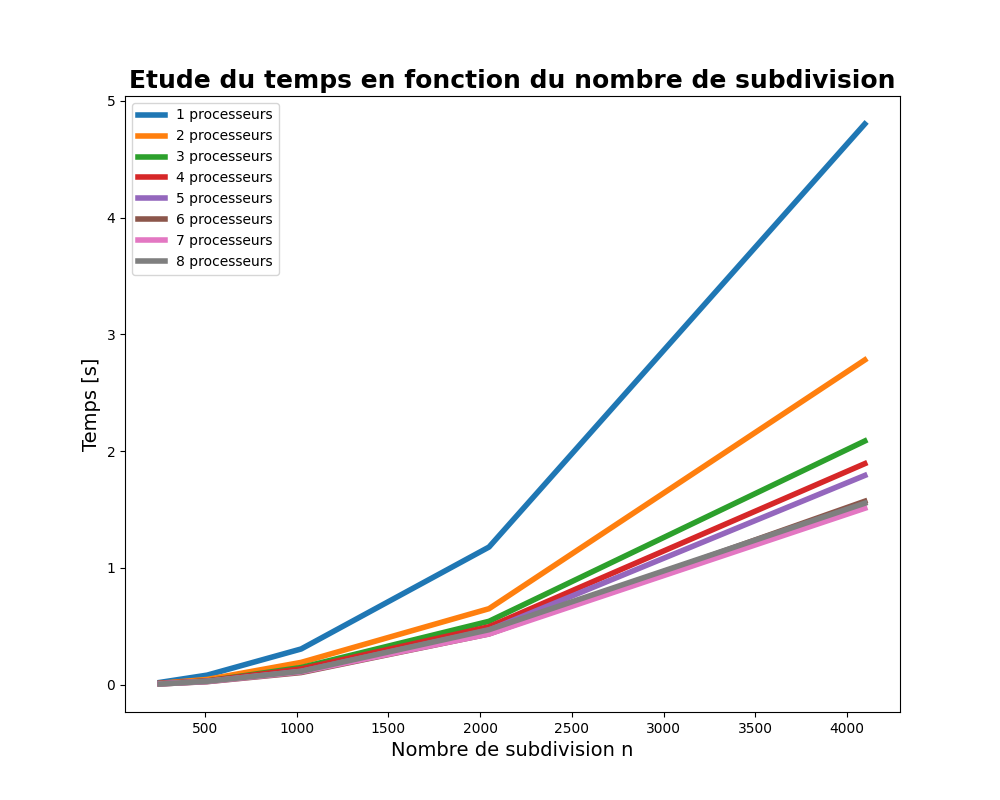
\includegraphics[width=0.45\linewidth]{../Images/time_gauss_Op_MP.png}}
  
    \caption{Méthode de Gaus 2D : Open MP}
    \label{fig:gaussMP}
  \end{figure}

\subsubsection{MPI}

\begin{figure}[H]
    \centering

    \subcaptionbox{Erreur \label{fig:errGaussMPI}}{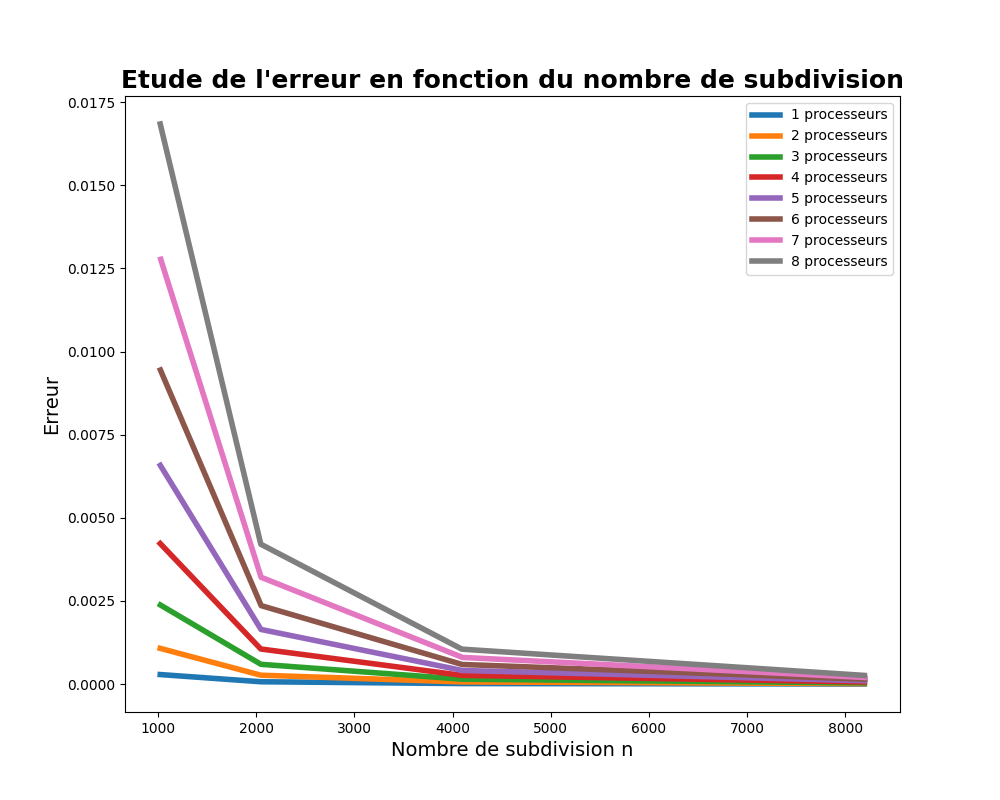
\includegraphics[width=0.45\linewidth]{../Images/error_gauss_MPI.png}}%
    \hfill % Ajoute une espace horizontale entre les sous-figures
    \subcaptionbox{Temps \label{fig:timGaussMPI}}{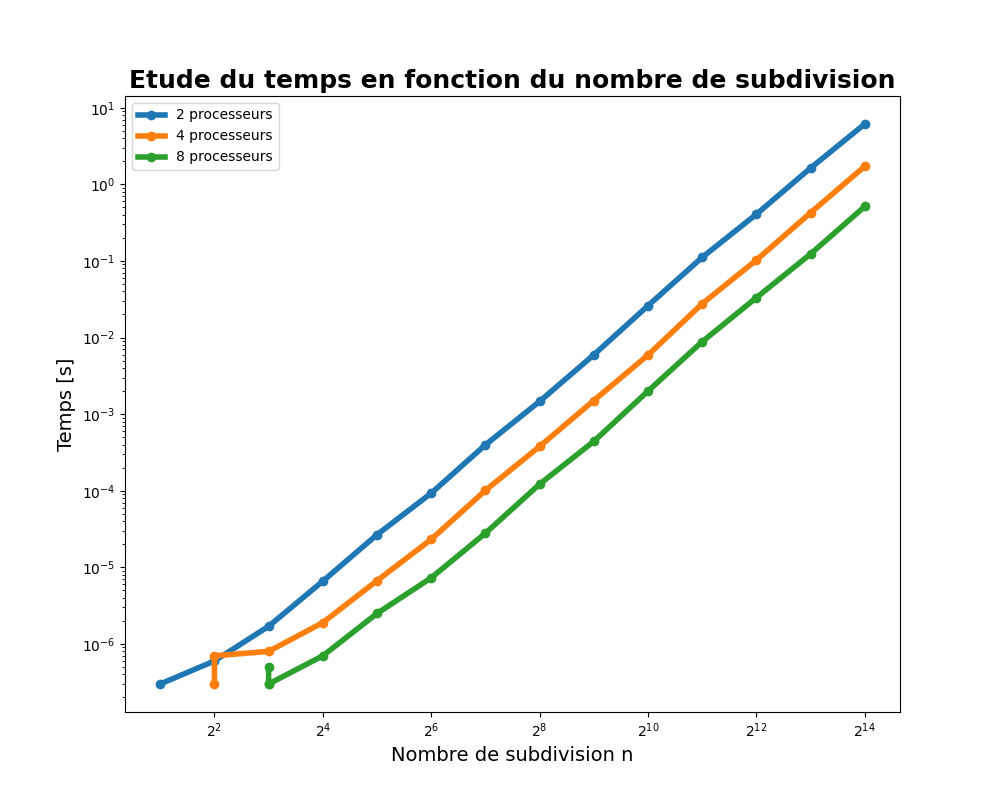
\includegraphics[width=0.45\linewidth]{../Images/time_gauss_MPI.png}}
  
    \caption{Méthode de Gauss 2D : MPI}
    \label{fig:gaussMPI}
  \end{figure}

\subsubsection{Cuda}
\begin{figure}[H]
    \centering

    \subcaptionbox{Erreur \label{fig:errSimpMPI}}{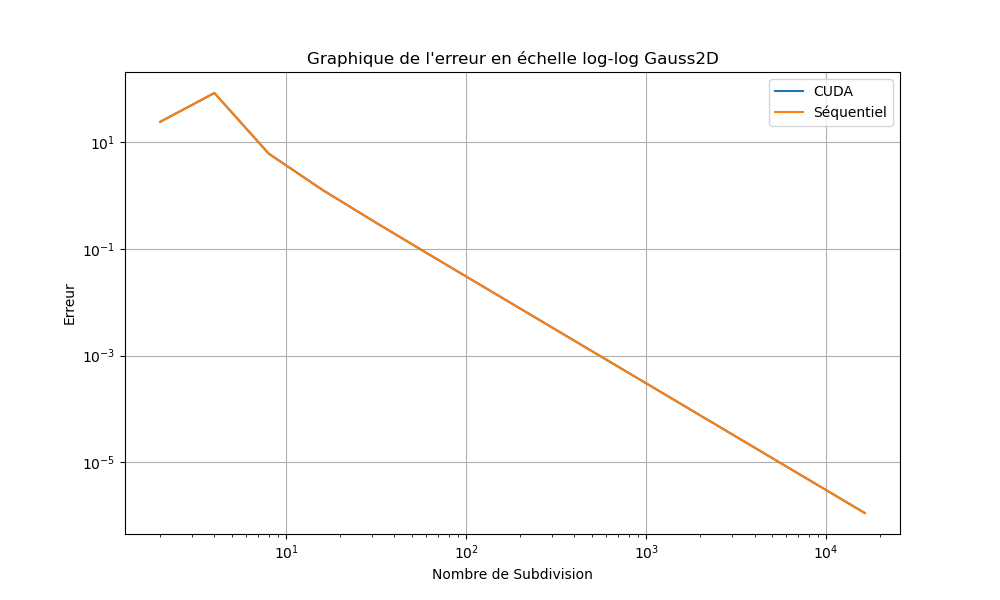
\includegraphics[width=0.45\linewidth]{../Images/error_Gauss2D_cuda.png}}%
    \hfill 
    \subcaptionbox{Temps \label{fig:timSimpMPI}}{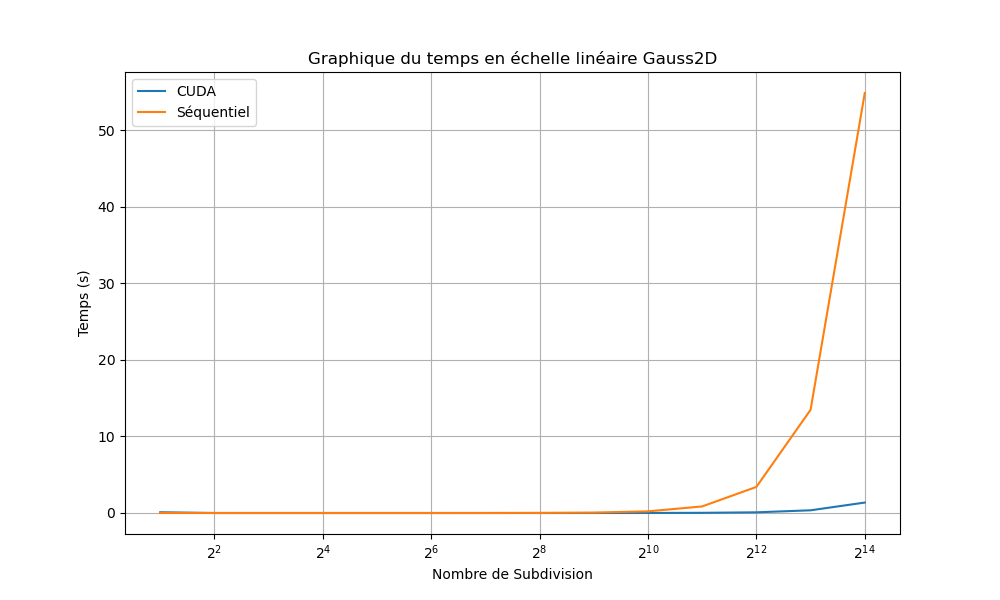
\includegraphics[width=0.45\linewidth]{../Images/time_Gauss2D_cuda.png}}
  
    \caption{Méthode de Simpson : MPI}
    \label{fig:simpMPI}
  \end{figure}

  \subsection{Monte Carlo} 

\subsubsection{Open MP}

\begin{figure}[H]
    \centering

    \subcaptionbox{Erreur \label{fig:errMCMP}}{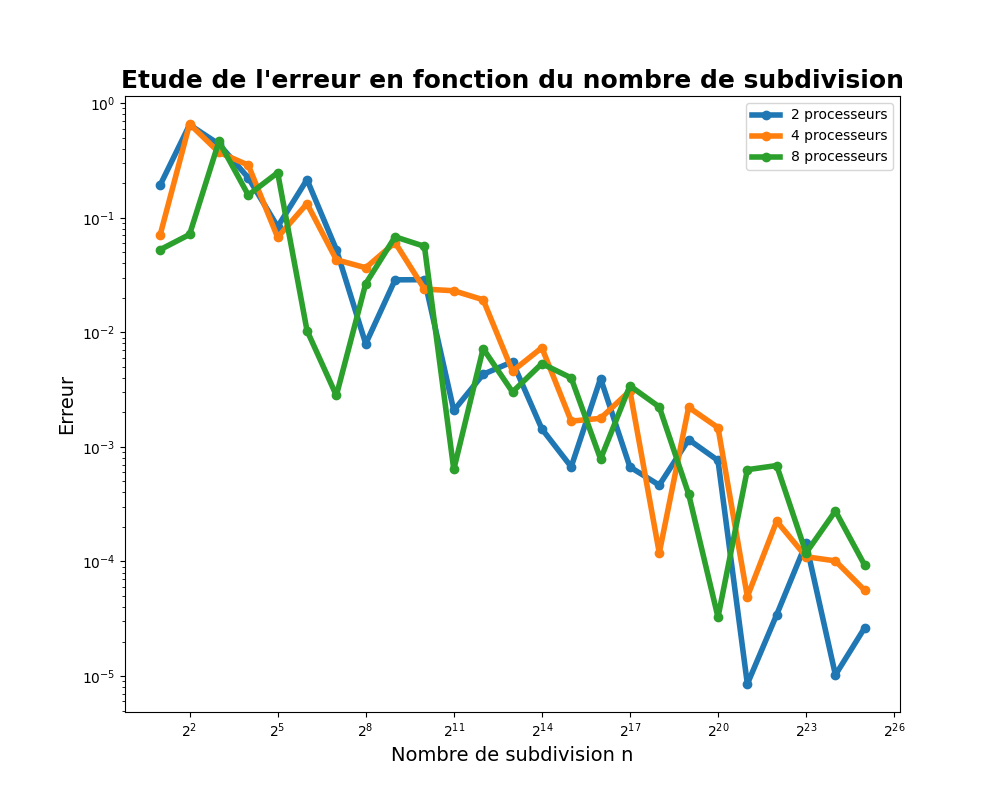
\includegraphics[width=0.45\linewidth]{../Images/error_montecarlo_Op_MP.png}}%
    \hfill % Ajoute une espace horizontale entre les sous-figures
    \subcaptionbox{Temps \label{fig:timMCMP}}{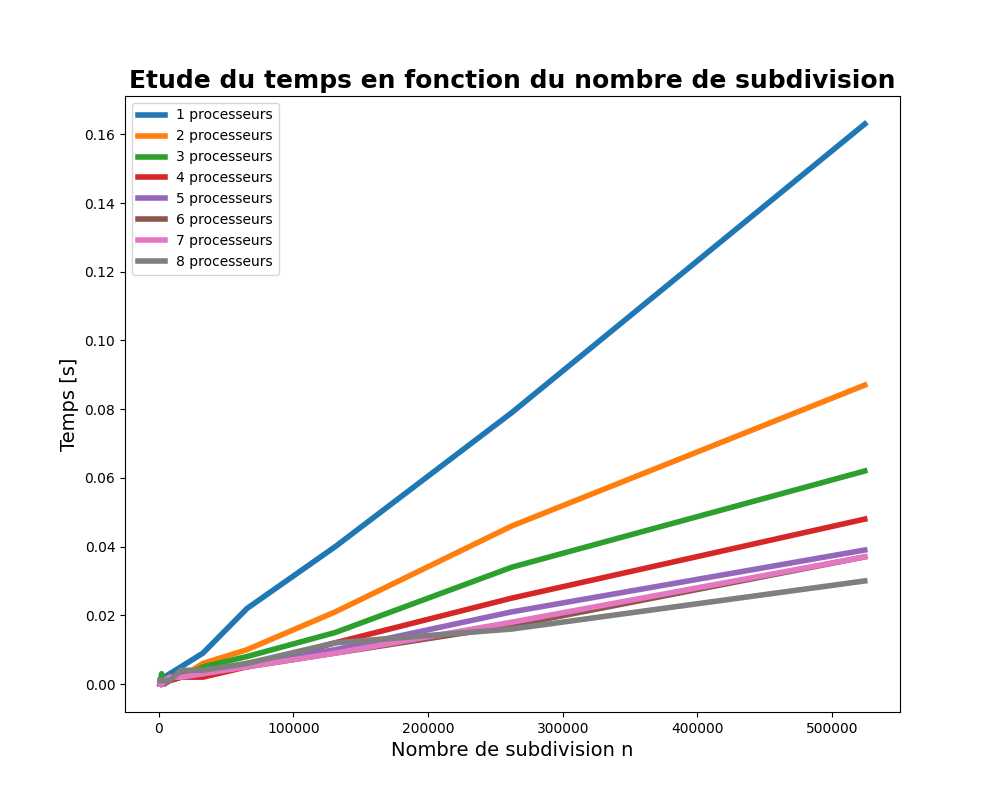
\includegraphics[width=0.45\linewidth]{../Images/time_montecarlo_Op_MP.png}}
  
    \caption{Méthode de Monte Carlo : Open MP}
    \label{fig:MCMP}
  \end{figure}

\subsubsection{MPI}

\begin{figure}[H]
    \centering

    \subcaptionbox{Erreur \label{fig:errMCMPI}}{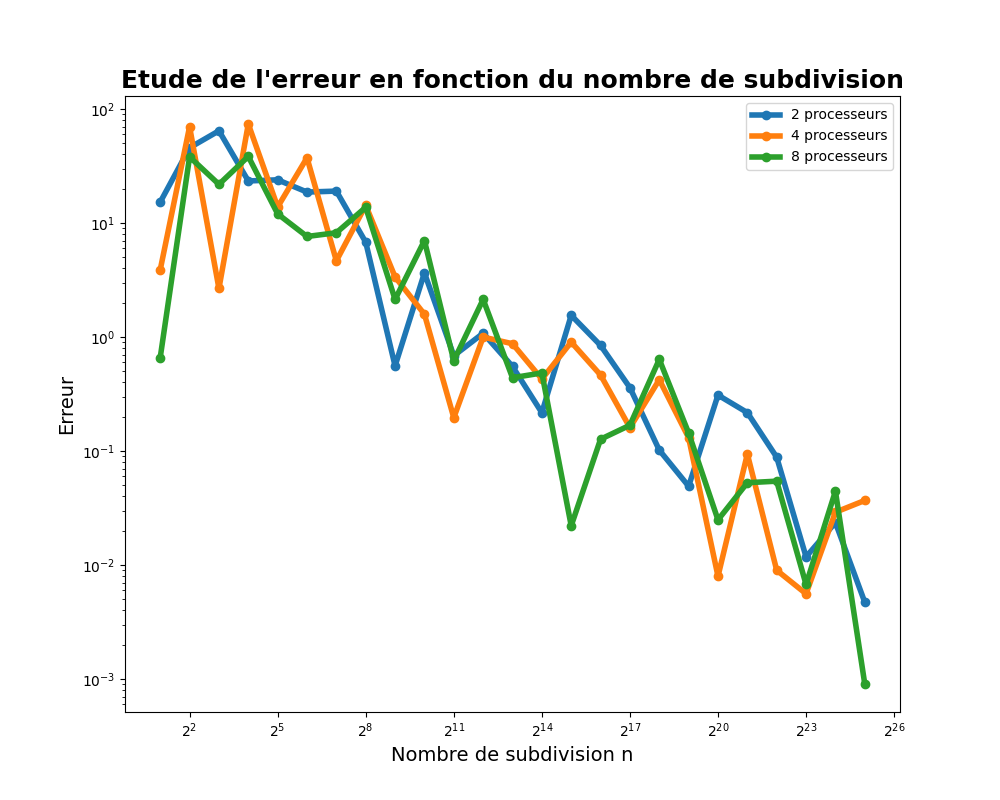
\includegraphics[width=0.45\linewidth]{../Images/error_montecarlo_MPI.png}}%
    \hfill % Ajoute une espace horizontale entre les sous-figures
    \subcaptionbox{Temps \label{fig:timMCMPI}}{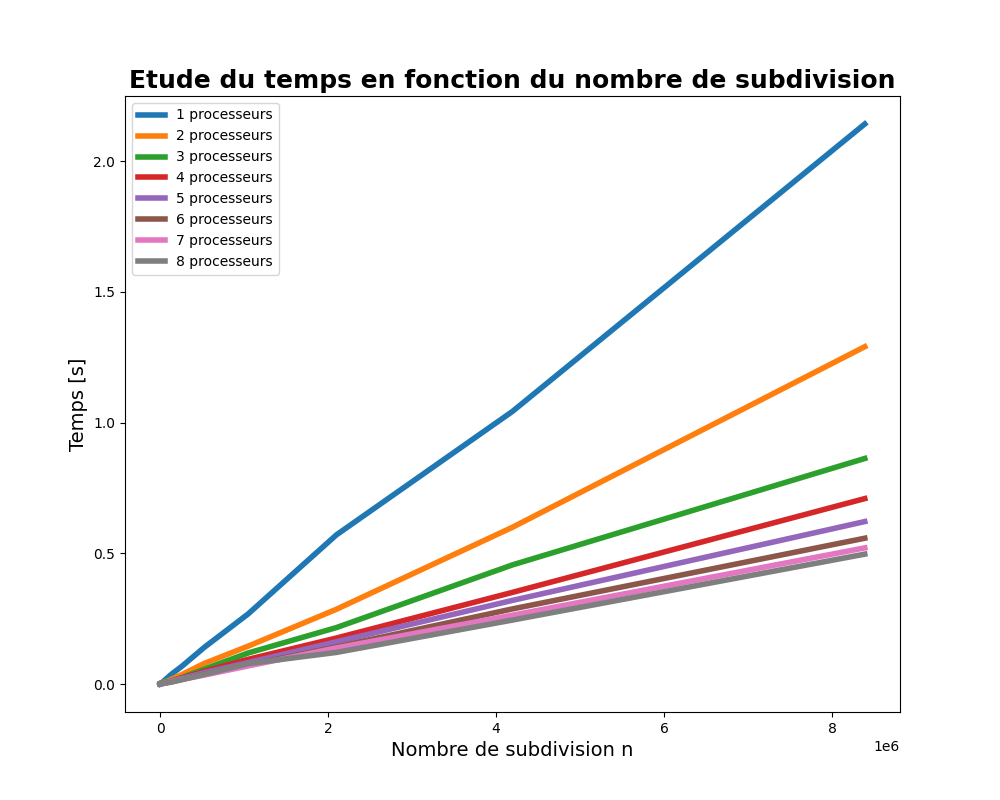
\includegraphics[width=0.45\linewidth]{../Images/time_montecarloMPI.png}}
  
    \caption{Méthode de Monte Carlo : MPI}
    \label{fig:MCMPI}
  \end{figure}

\subsubsection{Cuda}
\begin{figure}[H]
    \centering

    \subcaptionbox{Erreur \label{fig:errMCMPI}}{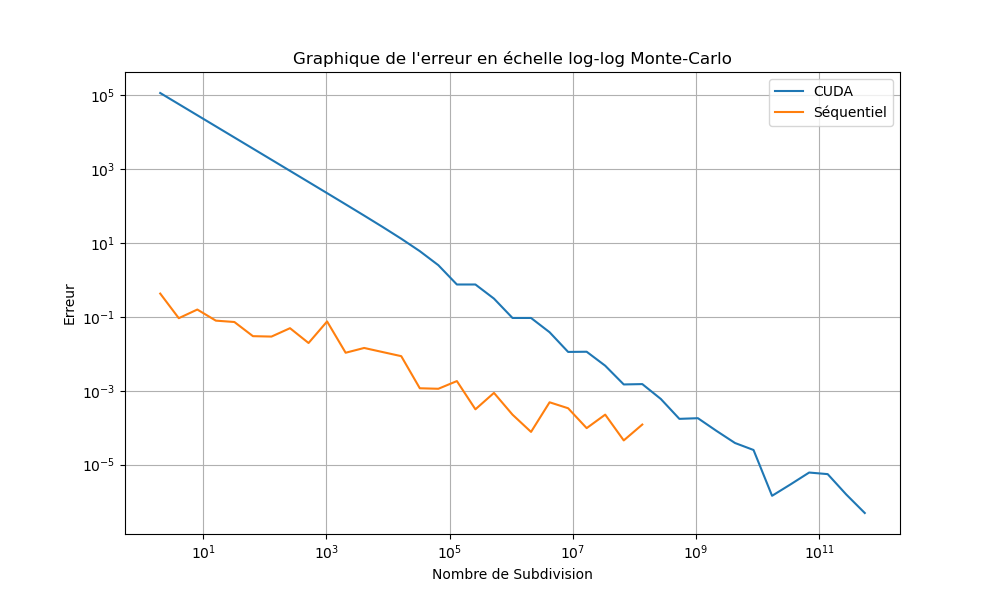
\includegraphics[width=0.45\linewidth]{../Images/error_monte_carlo_cuda.png}}%
    \hfill % Ajoute une espace horizontale entre les sous-figures
    \subcaptionbox{Temps \label{fig:timMCMPI}}{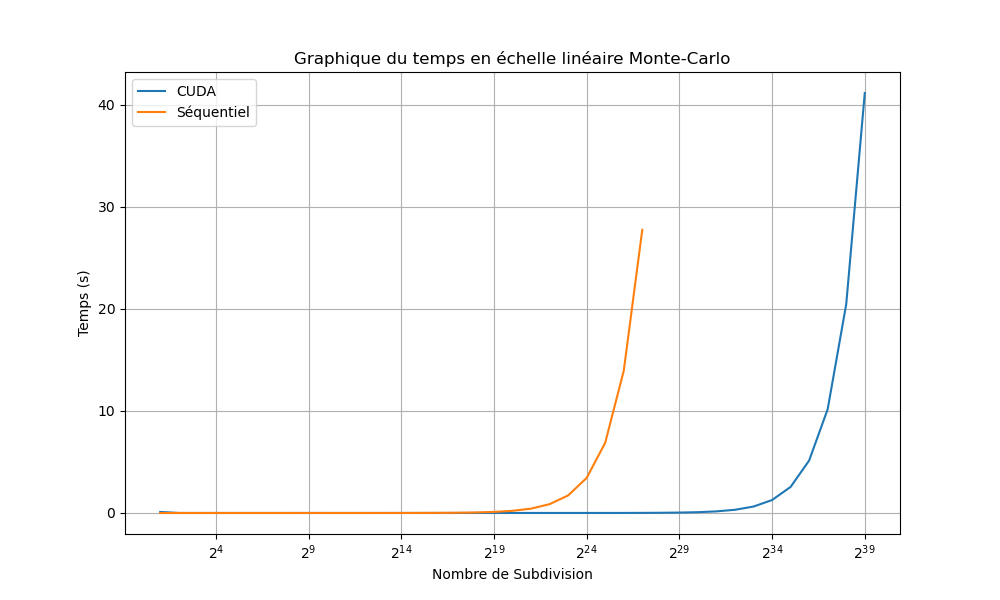
\includegraphics[width=0.45\linewidth]{../Images/time_monte_carlo_cuda.png}}
  
    \caption{Méthode de Monte Carlo : MPI}
    \label{fig:MCMPI}
  \end{figure}


\subsection{Analyse des résultats} \label{sec:analyse}
\subsection*{MPI - Open MP}
De manière générale, le temps de calcul pour chaque méthode croit en fonction du nombre de subdivisions. Cette croissance est plus faible quand on augmente le nombre de processeurs, mais ce gain et de moins en moins flagrant quand le nombre de processeurs atteint des valeurs élevées.

L'erreur diminue en fonction du nombre de subdivisions, mais il est plus difficile de tirer des conclusions sur son comportement en fonction du nombre de processeurs. 

Le comportement de l'erreur en fonction du nombre de processus peut varier.
Dans certains cas, l'erreur peut diminuer à mesure que le nombre de processus augmente, car cela permet de diviser le travail en tâches plus petites et donc potentiellement plus précises.
Cependant, une utilisation excessive de processus peut introduire des erreurs supplémentaires dues à des coûts de communication ou à des problèmes de synchronisation.

Pour approfondir l'analyse de chaque méthode et bibliothèque de parallélisation, examinons les détails suivants :

Pour la version \textbf{OpenMP} de \textbf{Simpson}, bien que l'erreur puisse sembler chaotique, elle demeure extrêmement faible. Une perspective intéressante consisterait à générer un graphique similaire avec une fonction présentant une erreur plus significative, afin d'étudier son comportement.

En ce qui concerne la version \textbf{MPI} de \textbf{Simpson}, une faible erreur est également observée. Une erreur plus importante pour un faible nombre de subdivisions pourrait résulter des coûts de communication entre les processus.

Dans la version \textbf{OpenMP} de \textbf{Gauss2D}, l'erreur est cohérente en fonction du nombre de threads, et elle décroît conformément au nombre de subdivisions, comme prévu.

En ce qui concerne la version \textbf{MPI} de \textbf{Gauss2D}, un coût de communication entre les processus est clairement perceptible, avec une légère détérioration de l'erreur lorsque le nombre de processus augmente.


Pour la méthode \textbf{Monte-Carlo}, les résultats des versions \textbf{OpenMP} et \textbf{MPI} sont conformes aux attentes. Étant donné que la méthode repose sur des probabilités, l'erreur peut être imprévisible pour un faible nombre de points, mais diminue rapidement avec leur augmentation.

\subsection*{Cuda}
\begin{itemize}
    \item \textbf{Méthode de Simpson :} Pour cette méthode, on observe une amélioration légère mais non significative de l'erreur avec CUDA. Dans les deux cas, parallélisé et séquentiel, l'erreur converge rapidement vers des valeurs de l'ordre de $10^{-14}$ à $10^{-15}$. Cependant, le temps de calcul avec CUDA devient plus long lorsque le nombre de subdivisions est suffisamment grand. Cette augmentation du temps de calcul s'explique par le fait que le nombre de blocs reste constant indépendamment du nombre de subdivisions. Une adaptation du nombre de blocs en fonction du nombre de subdivisions aurait été nécessaire, ou une augmentation du nombre de threads par bloc aurait pu être envisagée pour optimiser les performances.
    \item \textbf{Méthode Gauss2D} L'erreur demeure identique dans les deux cas, cependant, la version parallélisée avec CUDA se distingue par une nette accélération, particulièrement notable pour un nombre très élevé de points.
    \item \textbf{Méthode Monte-Carlo :} L'erreur est légèrement plus importante avec CUDA, mais elle décroît significativement plus rapidement que dans la version séquentielle. De plus, la version séquentielle atteint rapidement ses limites en termes de temps de calcul, tandis qu'avec CUDA, ce problème survient seulement pour des valeurs extrêmement élevées ($2^{39}$). Il est crucial de noter que la génération de nombres aléatoires sur CPU n'est pas réalisée de la même manière que sur GPU.
\end{itemize}
En somme, bien que chaque méthode ait réagi différemment à la parallélisation avec CUDA, l'utilisation de cette technologie s'avère prometteuse pour accélérer significativement les calculs numériques, surtout lorsque des volumes de données importants sont impliqués. Cette accélération des calculs, particulièrement observée dans les méthodes Gauss2D avec l'utilisation de CUDA, souligne l'intérêt de cette technologie lorsque l'objectif est de minimiser l'erreur numérique. La capacité à traiter des volumes de données importants dans des délais raisonnables offre la possibilité de réaliser des simulations avec des valeurs numériques élevées, facilitant ainsi la réduction de l'erreur associée aux calculs numériques. Cela renforce l'attrait de CUDA dans un contexte où la précision des résultats est cruciale.

\newpage
\section{Quelques explications du code}


\subsection{Exécution MPI - Open MP}

Entrez dans le fichier \verb|parametres_Machine| le nombre de processeur max que vous souhaitez utiliser.

Des scripts bash sont disponibles dans le dossier `Bashs`, ils permettent de lancer les codes pour chaque méthode et chaque paralélisation : 
\begin{itemize}
  \item Simpson : 
  \item Gauss2D :
  \item MonteCarlo 
\end{itemize}

Ces bashs compilent et executent le code $C_{++}$ pour une méthode et une parallélisation donnée et plottent les graphes de l'erreur et du temps d'execution à l'aide des données obtenues dans le dossier \verb|Results|. Les graphes sont sauvegardés dans \verb|Images|. L'utilisation de ces bashs requier la création d'un dossier \verb|Results| et d'un dossier \verb|Executables|.


Des scritps PowerShell sont également disponibles dans le dossier \verb|PowerShell| afin de pouvoir éxécuter les codes sous Windows.
\newline
Le fichier \verb|graph.py| dans le sous répertoire \verb|CodesPython| permet d'afficher les données dans le répertoire \verb|Results|. 
Il prend en entrée le nom préfix des données que vous voulez afficher.
Par exemple pour afficher les données pour la méthode de Simpson avec Open MP, placez vous dans le répertoire \verb|CodesPython| et tappez : 
\begin{center}
\verb|python3 graph.py "simp_Op_MP"|
\end{center}
Le code pour la méthode de Gauss 2D utilise la librairie Eigen, il sera nécessaire de linker la librairie et donc de devoir modifier légèrement les fichiers \verb|gauss2DMPI.cpp|, \verb|gauss2DOpenMP.cpp| ainsi que \verb|Gauss2D.cpp|.

\subsection{Exécution Cuda}
Pour chaque méthode, un script PowerShell est fourni et est construit de la manière suivante :
\begin{itemize}
\item Exécution du programme CUDA.
\item Exécution du programme non parallélisé.
\item Exécution du programme graph\_cuda.py pour enregistrer les graphiques.
\item Suppression des fichiers générés pendant la compilation et des fichiers txt nécessaires au programme Python.
\item Déplacement des graphiques dans le dossier Images.

\end{itemize}

La librairie Eigen est fournie dans le dossier cuda pour éviter tout problème de bibliothèques.

\newpage
\section{Conclusion - Perspective}
Ce projet a permis d'explorer et de comparer différentes méthodes de calcul numérique, en mettant particulièrement l'accent sur la parallélisation avec OpenMP, MPI et CUDA. Chaque méthode a ses avantages et ses inconvénients, et le choix de la parallélisation dépend largement de la nature du problème et des ressources matérielles disponibles.

L'utilisation d'OpenMP pour paralléliser des tâches sur CPU offre une approche simple et efficace pour exploiter les capacités multi-cœurs des processeurs. MPI, en revanche, offre une solution robuste pour la programmation parallèle distribuée sur des clusters de machines. La parallélisation avec CUDA sur GPU offre une puissance de calcul massive, mais nécessite une gestion minutieuse de la mémoire et une compréhension approfondie de l'architecture GPU.

Les résultats obtenus ont montré que la parallélisation peut considérablement réduire le temps d'exécution des calculs, en particulier pour des problèmes complexes nécessitant une grande puissance de calcul. Cependant, il est important de noter que l'efficacité de la parallélisation dépend du problème spécifique et de la capacité du matériel.

En conclusion, ce projet a permis d'acquérir une expérience pratique dans la mise en œuvre de différentes méthodes de calcul numérique et de comprendre les nuances de la parallélisation. Il offre également une base solide pour explorer davantage les possibilités de parallélisation dans d'autres contextes et pour d'autres types de problèmes.

En perspective, il serait nécessaire d'adapter les codes existants et de créer des scripts bash permettant l'utilisation de plusieurs fonctions de test. Par ailleurs, une optimisation plus poussée de la gestion du nombre de blocs et de threads sur CUDA s'avérerait indispensable. Il aurait également été enrichissant d'explorer diverses distributions et de les évaluer sur un éventail de fonctions dans le contexte de la méthode Monte-Carlo, afin d'obtenir une compréhension approfondie de leur impact sur les résultats.

\end{document}